\documentclass[12pt]{standalone}
\usepackage{tikz}

\begin{document}

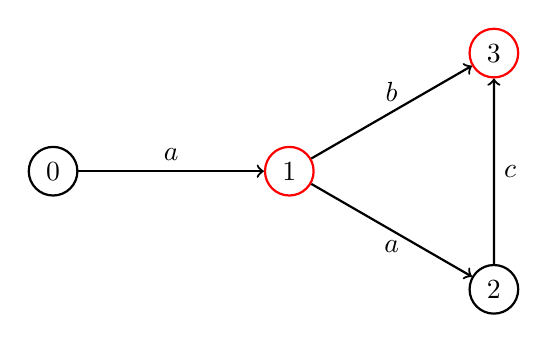
\begin{tikzpicture}[thick,scale=1.5]
    \node[draw=black,fill=none,circle] (0) at (-2,0) {$0$};
    \node[draw=red,fill=none,circle] (1) at (0,0) {$1$};
    \node[draw=black,fill=none,circle] (2) at (1.732,-1) {$2$};
    \node[draw=red,fill=none,circle] (3) at (1.732,1) {$3$};
    \path (0) edge[->] node[pos=0.5,above] {$a$} (1);
    \path (1) edge[->] node[pos=0.5,below] {$a$} (2);
    \path (2) edge[->] node[pos=0.5,right] {$c$} (3);
    \path (1) edge[->] node[pos=0.5,above] {$b$} (3);
\end{tikzpicture}

\end{document}
